
\documentclass{article}
\usepackage{amsmath, amssymb, fullpage, dsfont, graphicx, float, verbatim, bm, hyperref}


\begin{document}

\title{STA 841 Categorical Data Analysis \\ Predict'em All}
\author{Sarah Normoyle, Gonzalo Bustos}
\date{\today}
\maketitle


\section{Introduction}

PokemonGo is a augmented virtual reality game that came out in July 2016 where a player can catch, train, and fight creatures called Pokemon. These Pokemon appear randomly based on GPS location in the game as if they were in the same location as the player. Pokemon appear and disappear for varying time lengths. There are theoretically 151 species of Pokemon that can appear in the game, with some being much more common than others. These species can be classified into types, with some classified into more than one type. In addition to Pokemon, there are also Pokestops and Gyms based on GPS location in the game. Players can collect items such as Pokeballs at Pokestops and can train and fight Pokemon in Gyms. Because PokemonGo is a game, there is an underlying algorithm that produces Pokemon spawns. Without knowing the algorithm or the random distribution of Pokemon, we seek to find insight into how Pokemon are distributed. 


\section{Data}

The dataset used for this project is from kaggle.com and can be found at \hyperlink{Ref1}{[1]}.  The data set has about 300,000 observations of Pokemon sightings in the game PokemonGo from all over the world. Each observation in the dataset contains information about the sighting, including which Pokemon and location, time, and weather variables. We also collected data on which type each Pokemon is from the reference \hyperlink{Ref2}{[2]} . For the sake of simplicity and interpretation, we only considered a Pokemon's first type, which is traditionally used to sort Pokemon. We also have variables related to each Pokemon's stats and total stats, which we could also consider as a response variable. Variables that we will consider as covariates include: close to water (Boolean), distance to nearest Pokestop and nearest Gym, population density, terrain type (according to \hyperlink{Ref3}{[Ref 3]} about MODIS Land Cover), temperature, and time of day (in 24 hour period). Additionally, based on latitude and longitude, we added a couple variables, which are City and Country.

\section{Research Question}

The ultimate question of the game is being able to predict the next location of a Pokemon. This would require investigating the spatio-temporal relationship of Pokemon spawns, as well as other time and location specific variables. In addition to this question, another interesting question for players is what is the probability of observing a particular Pokemon or a particular type of Pokemon, especially a rare type. Given that our data set is non-uniform sample of exclusively observations of Pokemon, we will address the following question:

\begin{itemize}

	\item Given that a Pokemon appears, what factors are related to the probability of observing a particular type of species of Pokemon?

\end{itemize}

\section{Exploratory Data Analysis}

The data set contains 296,021 observations from 9/2/2016 to 9/8/2016. About half of the observations are within the United States, and the other observations are scattered around the globe. The frequency of each type of Pokemon is different based on our non-representative sample and also based on how often they appear in the game. First we look at the counts per type of Pokemon.

\begin{figure}[H]
\centering
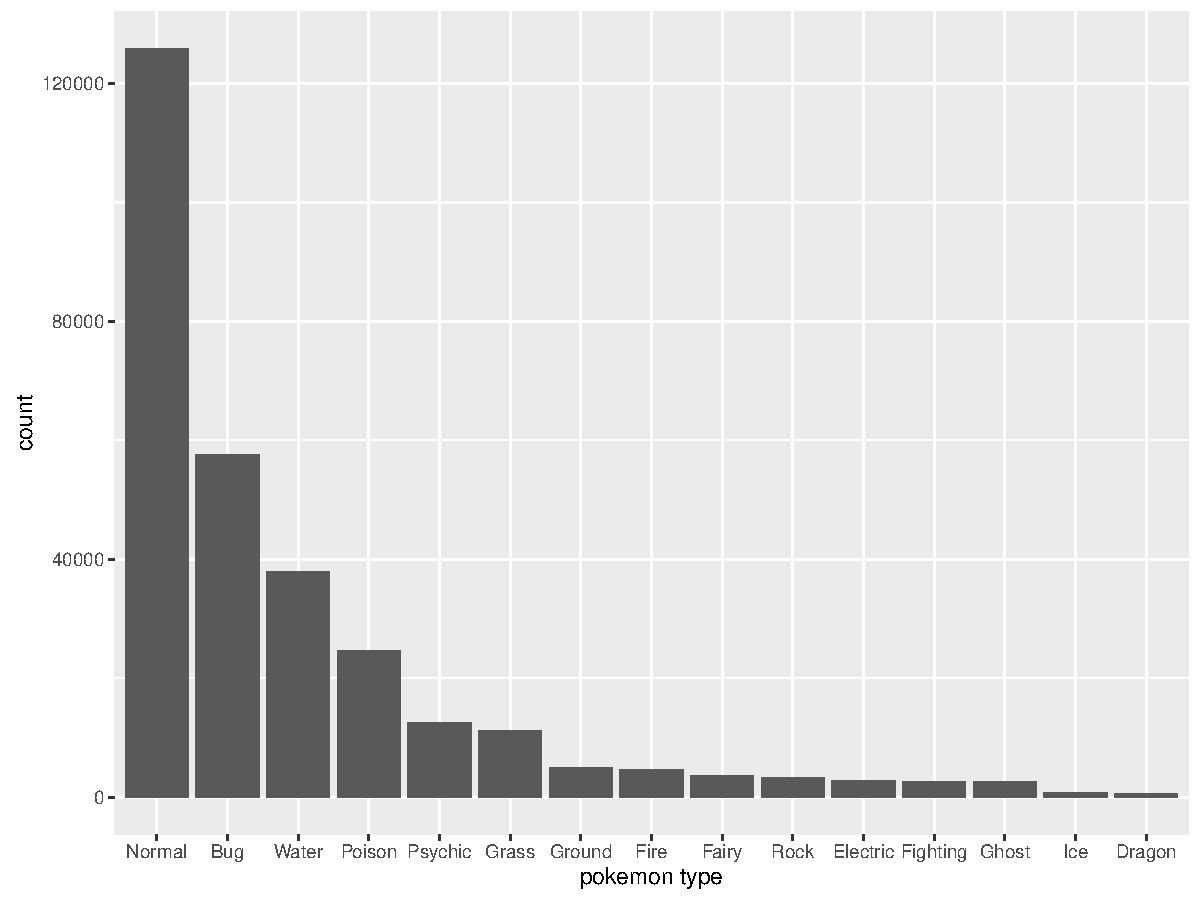
\includegraphics[scale = 0.4]{count_by_type.pdf}
\caption{Frequency Counts of Pokemon}
\end{figure}

\noindent It is clear that the frequency of types are not uniform. However, our question is if the distribution of species changes based on other variables. We will consider location, time, and weather variables as potential covariates and explore the relationships among the variables.

\subsection{Location}
When looking at location as a potential covariate, we first look at where the observations in our dataset occur. Below is a heat map plot of just the United States.

\begin{figure}[H]
\centering
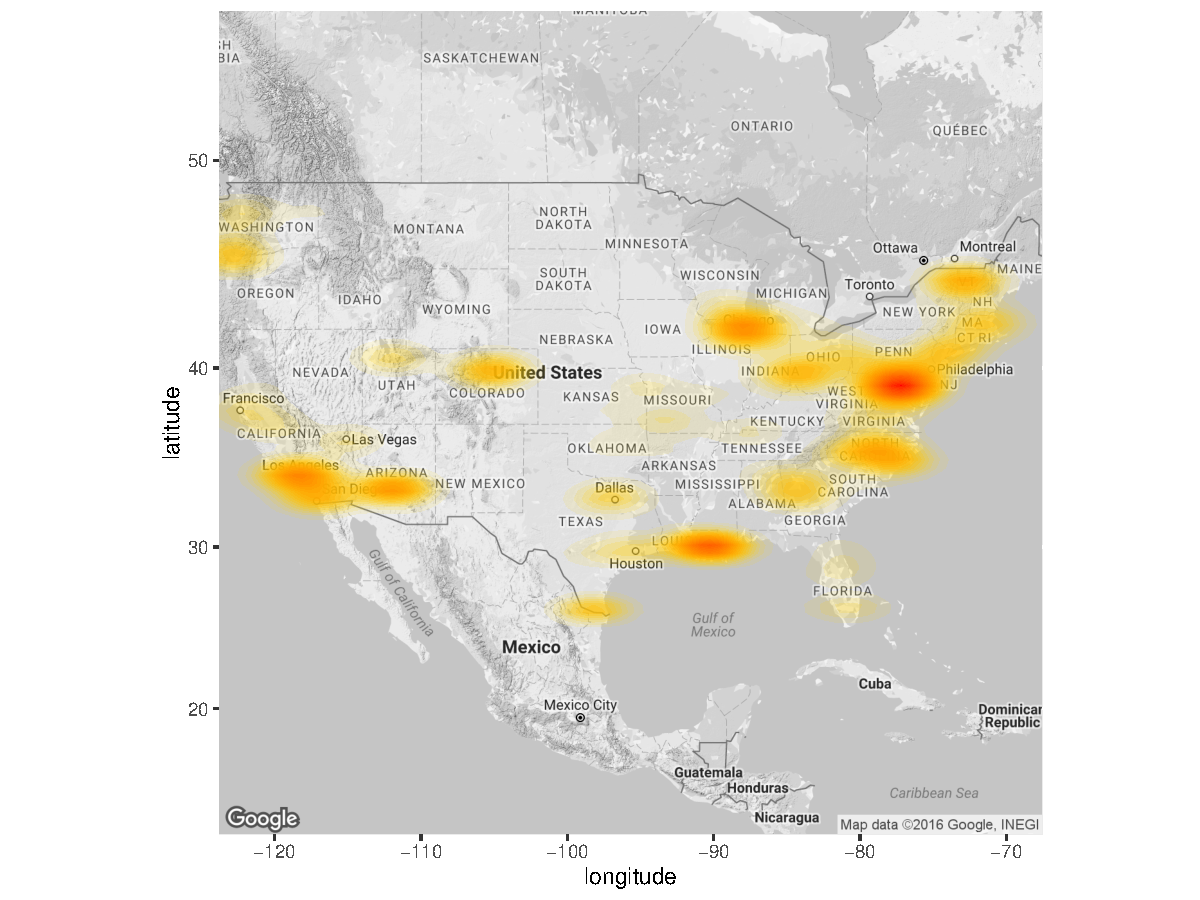
\includegraphics[scale = 0.45]{heatmap.pdf}
\caption{Heat Map of United States Pokemon Counts}
\end{figure}

\noindent After looking at this plot, we believe that our sample of data is neither a representative nor a random sample of Pokemon seen during the time period because certain parts of the country have no points and some parts of the country are over-sampled. Because we are focusing on comparing how species distribution changes among the sample, this is not concerning. Below is another plot showing the difference in distributions across species for terrain types and distance to water.

\begin{figure}[H]
\centering
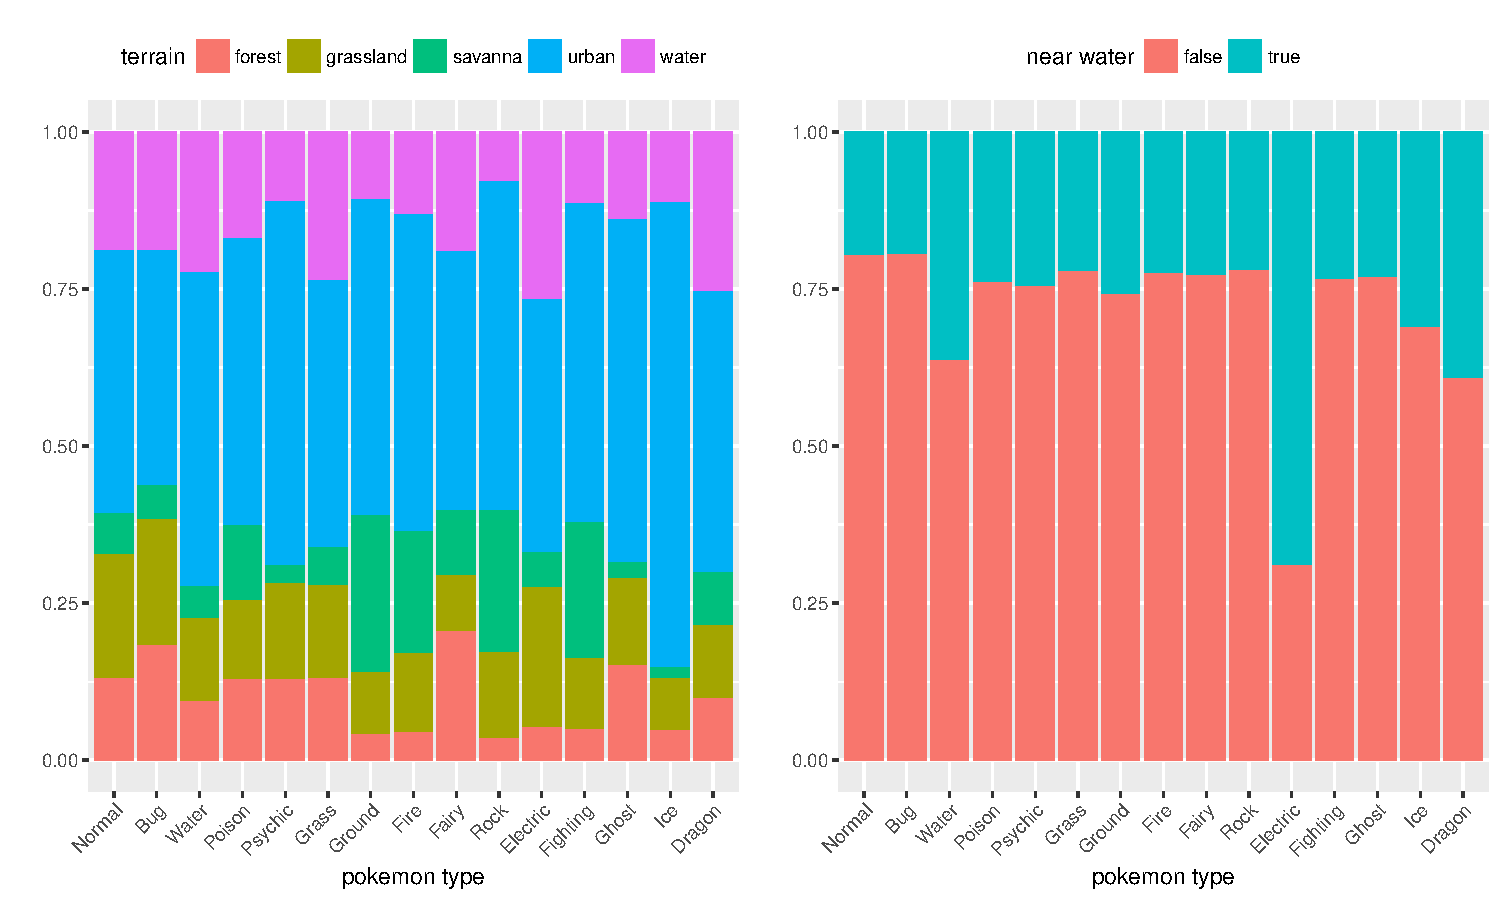
\includegraphics[scale = 0.5]{side_by_side_plot.pdf}
\caption{Terrain Types and Distance to Water}
\end{figure}

\noindent On the y-axis of these plots is the proportion of counts, and on the x-axis is type of Pokemon. There seems to be a relationship between terrain type and proportion of species as well as distance to water and proportion of species. For distance to water, of the Pokemon found close to water, there are more water and electric Pokemon for example. In addition, population density is also a variable that relates to the presence of a particular species. Perhaps certain types appear more where it is more/less dense.

\subsection{Time and Weather}

Because this sample of data is only over the course of 6 days, the main variable we can look into is time of day. From intuition, perhaps certain types of Pokemon are more or less likely to appear at night than other types of Pokemon. In addition, we investigated if weather had a relationship with type of Pokemon. Both time and weather did not seem to have a strong relationship with the distribution of Pokemon on their own, not when included in a final model.

\section{Model Methods}

\subsection{Binary Logistic Regression} 

First, each type of species was treated as a binary regression problem, which means either that type of Pokemon or not. Of the 15 types of Pokemon, the ones that were most investigated were Normal, Bug, Water, and Poison because they have the most counts. This analysis addresses the question of to what extent do certain time and location variables relate to the probability of seeing a particular type of Pokemon compared to the seeing the others. Predictors were first fit individually and then were added in a step-wise manner to create a full model for each Pokemon type. \\ 
\\ 
In addition to creating a model with fixed effects, we considered incorporating terms for random effects. These random effects capture additionally variation that is not captured by the current fixed effects. Random effects were added for the country of observation. 

\subsection{Multinomial Probit Regression}

After binary logistic regression, a multinomial probit model was also fit to the data that allows for a multinomial response, which would be the different types of Pokemon.

\section{Results}
Individual predictors had a different relationship with type of Pokemon. For example, for predicting Water vs. not water closeToWater had the biggest change in deviance and the lowest AIC. For Bug Pokemon, type of terrain had biggest change in deviance compared to the null model. When running stepwise regression, each additional variable added significantly changed the AIC value. The final model used for each binary regression of Pokemon:

\begin{center}
logit($\pi$) = $\beta_0$ + $\beta_1$ I(closeToWater) + $\beta_2$ I(pop:rural) + $\beta_3$ I(pop:suburban) + $\beta_4$ I(pop:urban) + $\beta_5$ I(gymin100m) + $\beta_6$ I(pokestopIn100m) + $\beta_7$ I(grassland) + $\beta_8$ I(savanna) + $\beta_9$ I(urban) + $\beta_{10}$ water + (1$|$Country)
\end{center}

\noindent The results after fitting 5 binary logistic regressions: \\ 
\\ 
\textbf{Fixed effect estimates:} \\ \\ 
\begin{tabular}{| l | c | c | c | c |}
	\hline
	Parameters & Normal Model & Water Model & Bug Model & Poison Model \\
	\hline 
	Intercept & -0.218 & -2.772 & -1.055 & -2.334 \\ 
	I(closeToWater) & -0.309 & 0.671 & -0.199 & 0.086 \\ 
	I(rural) & -0.011 & 0.061 & 0.037 & -0.240\\ 
	I(pop:urban) & -0.132 & 0.199 & -0.076 & 0.020 \\ 
	I(gymin100m) & 0.017 & 0.069 & -0.545 &  -0.072 \\ 
	I(pokestopIn100m) & -0.171 & 0.320 & -0.137 & 0.116 \\ 
	I(grassland) & 0.151 & 0.066 & -0.224 & -0.337 \\ 
	I(savanna) & -0.342 & 0.236 & -0.757 & 0.512 \\ 
	I(terr:urban) & -0.071 & 0.448 & -0.482 & -0.059  \\ 
	I(terr:water) & 0.034 & 0.574 & -0.310 & -0.192 \\ 
	\hline
\end{tabular} 
\\ 
\\ 
\\ 
\textbf{Random effect estimates:} \\ \\ 
\begin{tabular}{| l | c | c | c | c |}
	\hline
	& Normal & Water & Bug & Poison \\  
	\hline
	Country Variance & 0.1597 & 0.3637 & 0.1576 & 0.2278 \\ 
	\hline
\end{tabular} 
\\ 
\\ 
\\ 
There are numerous differences regarding the log odds coefficients between the various binary models. Some variables make a big difference in log odds for some Pokemon types while they don't make much of a difference for other Pokemon types. For example, the odds of seeing a water Pokemon go up in population dense, urban areas near the water and near Pokestops while the odds of seeing a bug Pokemon go up in not population dense, rural areas with forest terrain not near the water and not near Pokestops. In addition, the random effect for Country ranges from about -1 to 1 on most of the models and helps to explain much of the variation. Perhaps there are other variables that differ between countries, or perhaps the distribution of species simply differs that much between countries. 

\newpage
\noindent 4 data examples to show examples of probabilities from each of the 4 model estimates:  \\ 
\\ 
\begin{tabular}{| l | c | c | c | c |}
	\hline
	Covariates & 1 & 2 & 3 & 4 \\ 
	\hline
	closeToWater & true & false & false & true \\ 
	pop density & urban & rural & mid & urban \\ 
	gymin100m & true & false & false & true \\ 
	pokestopIn100m & true  & false & false & true \\ 
	terrain & water & forest & grassland & savanna \\ 
	country & Netherlands & Germany & Spain & UK \\ 
	\hline 
\end{tabular}
\\ 
\\ \\ 
Probabilities for each of 4 models for each of 4 example (bolded is biggest of the examples for that model): \\
\\  
\begin{tabular}{ | c | c | c | c | c |}
	\hline
	Model & 1 & 2 & 3 & 4\\ 
	\hline
	Normal & 0.3448 & \textbf{0.4776} & 0.4330 & 0.2903 \\
	Water & \textbf{0.5049} & 0.0573 & 0.0887 & 0.2030 \\ 
	Bug & 0.1189  & \textbf{0.3578} & 0.1738 & 0.1040 \\ 
	Poison & 0.0337 & 0.0536 & 0.1093 & \textbf{0.1197} \\ 	
	\hline
\end{tabular}\\ 
\\ \\
When the multinomial model was fit for the types, the fit is much worse because we are incorporating more types of Pokemon. The model always predicts a Normal Pokemon because this is the Pokemon with the highest mean probability. This type of model would need more work and more variables to be able to distinguish situations in which the other Pokemon were more probable. Overall, the models do not do well in predicting which Pokemon will appear given the data. However, we are able to see when the odds of seeing a Pokemon increases or decreases.

\section{Limitations}

A limitation with this data set is the non-uniform sampling of Pokemon. Because the occurrences of Pokemon are a random sample over time and location, we are not able to model the rate of Pokemon appearances. In addition, because the Pokemon are not sampled uniformly and because we only have presence and not absence data, it is more difficult to model the occurrence of all Pokemon. \\ 
\\ 
However, despite this unequal sampling scheme, we are able to conduct an the analysis of differences between occurrences of types of species. The concern for sampling bias here would be if times or locations with a particular type of species were oversampled compared to the other types. However, if we control for the factors that introduce this sampling biases (such as population density) we are able to make observations about differences between types of species. 

\section{Conclusion and Extensions}

Based on our analysis, there appears to be a small relationship between location and the distribution of types of species in PokemonGo, and these covariates relate to each of the species differently. We could continue this analysis to do further model comparisons, and explore additional models and covariates. There are also many potential further explorations of this dataset and PokemonGo that could be investigated. It is most likely that Pokemon spawns are not independent observations and are dependent on other Pokemon's spawn time and location. Therefore, building a spatio-temporal dependency structure could be beneficial for the model. 

\newpage
\section{References}

\hypertarget{Ref1}{[1] \url{https://www.kaggle.com/semioniy/predictemall}.}

\noindent \hypertarget{Ref2}{[2] \url{http://bulbapedia.bulbagarden.net/wiki/List_of_Pokemon_by_National_Pokedex_number}.}

\noindent \hypertarget{Ref3}{[3] \url{http://glcf.umd.edu/data/lc/}.}

\noindent \hypertarget{Ref4}{[4] http://stackoverflow.com/questions/14334970/convert-latitude-and-longitude-coordinates-to-country-name-in-r}.

\section{Appendix: R Code}

\subsection{coords2country}
From Reference [4].

\verbatiminput{coords2country.R}

\subsection{Cleaning}
\verbatiminput{EDA.R}

\subsection{EDA}
\verbatiminput{initial_map_113016_v3.R}

\subsection{Models}
\verbatiminput{models.R}


\end{document}